%! Author = nail
%! Date = 09/03/2023

% Preamble

\chapter{Programmation}
\setcounter{chapter}{1}

% Document
\begin{article}
    \section{Préambule}\label{sec:preambule}%
    Pour implementer le modèle de Potts, nous allons suivre le schema que nous avons mis en place afin de pouvoir générer des modèles le plus simplement possible.
    \newline On a donc diviser les taches selon ce schema :
    \newline
    \begin{figure}[ht]
        \centering
        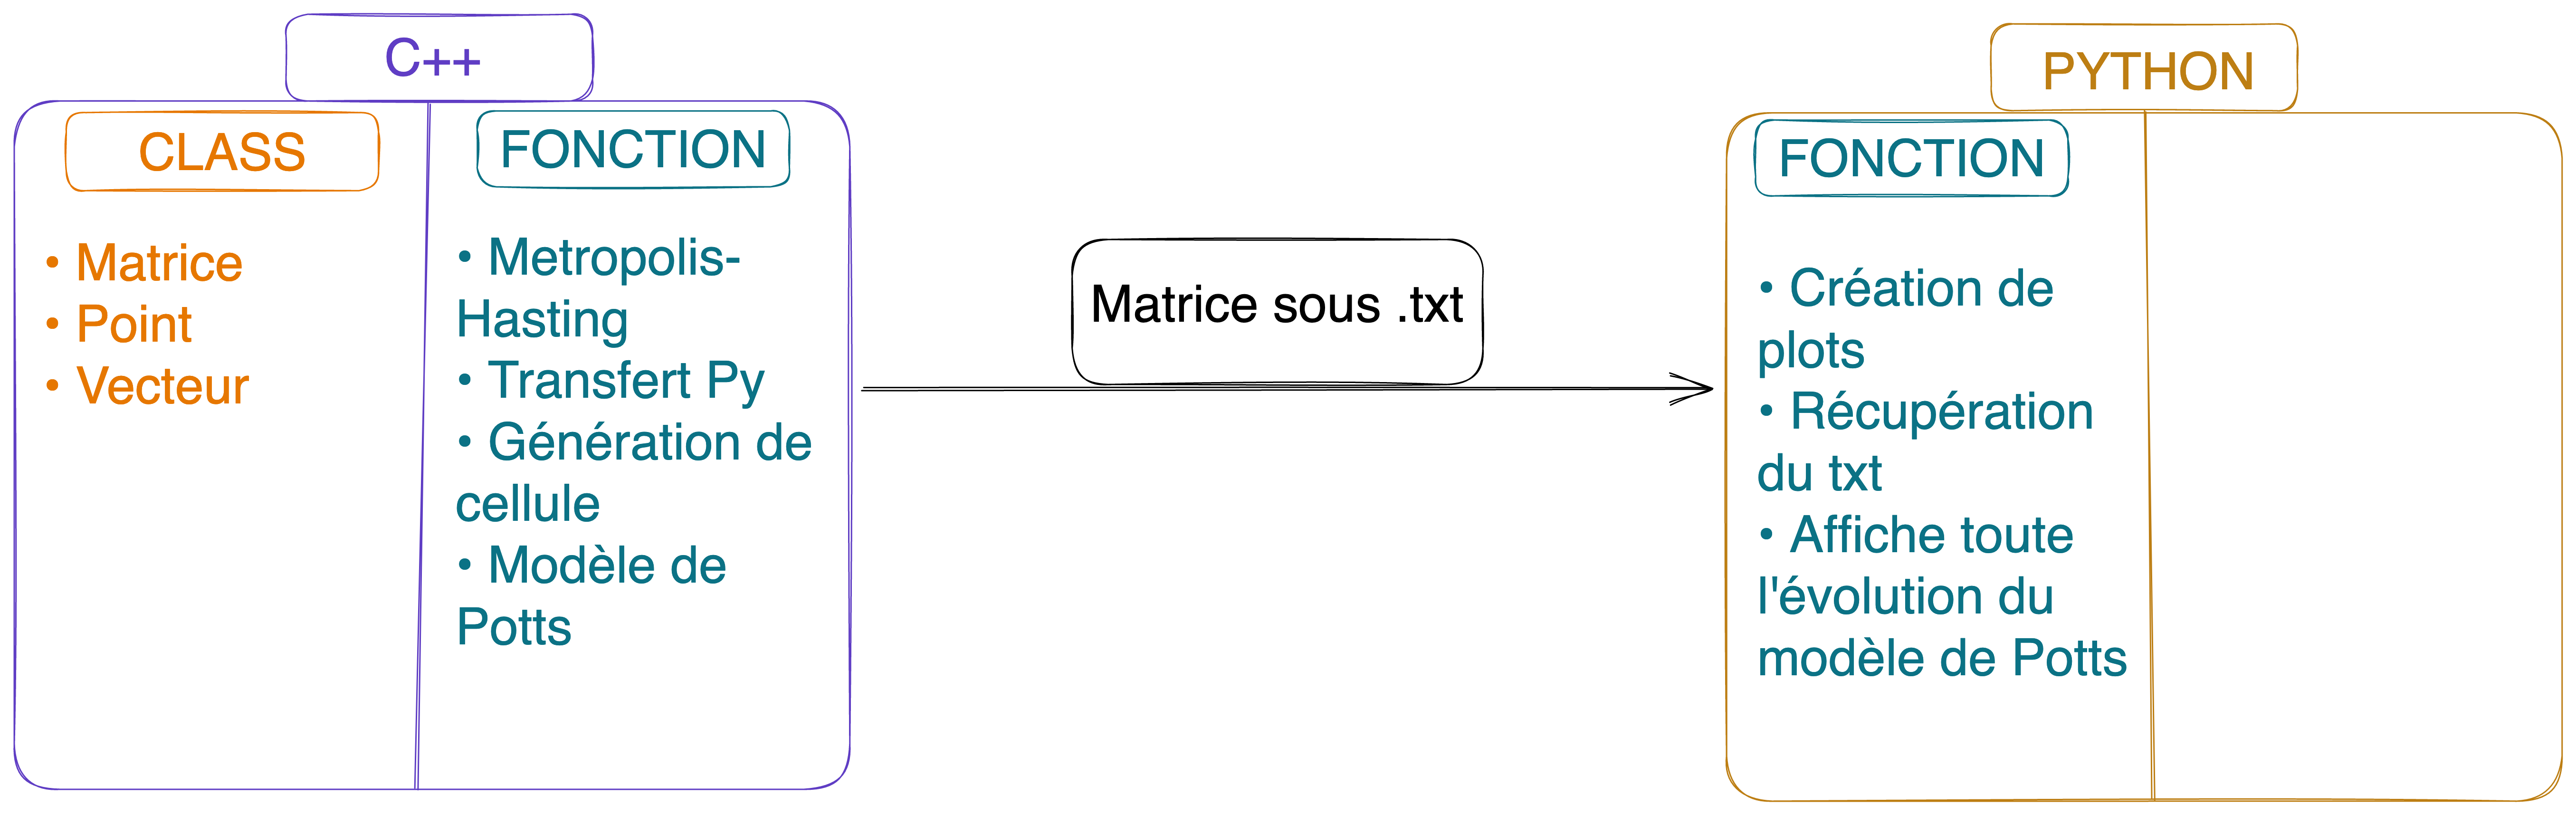
\includegraphics[scale=0.09]{./img/prog/Schema_prog}
        \caption{Schema de programmation}
        \label{fig:prog1}
    \end{figure}

    On a, selon ce schema, deux langages de programmation différents le C++ et le Python.

    \section{Explication}\label{sec:explication}
    \subsection{Préambul en C++}\label{subsec:preambul-en-c++}
    \noindent On va donc implémenter 3 classes différentes :
    \begin{description}
        \item[point] Une classe de point avec 2 coordonnées dont chacun ont un état, dans cette classe nous aurons des fonctions qui modifieront les propriétes des points.
        \item[matrice] Cette classe va nous permettre d'avoir une matrice de point.
        \item[vecteur-template] Ce n'est pas vraiment une classe, car ici nous allons utiliser la classe deja présente en C++, vector\footnote{Documentation officielle de la classe sur : https://cplusplus.com/reference/vector/vector/}.
        Nous allons ainsi ajouter des fonctions propres à cette classe pour pouvoir l'utiliser avec les points.
    \end{description}
    \newline
    \newline
    On pourra donc grâce à ces classes implementer le modèle de Potts.
    \newline On a choisis de faire des classes et donc de se rajouter une charge de travail au debut car cela semblait plus approprié et nous permettait aussi de parfaire notre niveau de programmation dans le langage C++.

    \subsubsection{Classe point :}

    Pour la classe point on crée un objet avec trois principaux attributs : ses deux coordonnées et son état.
    \newline On ajoute des fonctions qui permettent de modifier les attributs pour plus tard.
    La classe est surtout utile pour la modélisation et l'affichage sur un graphique qu'on verra après.
    \newline On y ajoute aussi les fonctions telles que la comparaison d'états entre deux sommets par exemple..
    Le fichier header de la classe point se présente comme ça :
    \newpage
    \begin{figure}[t]
        \centering
        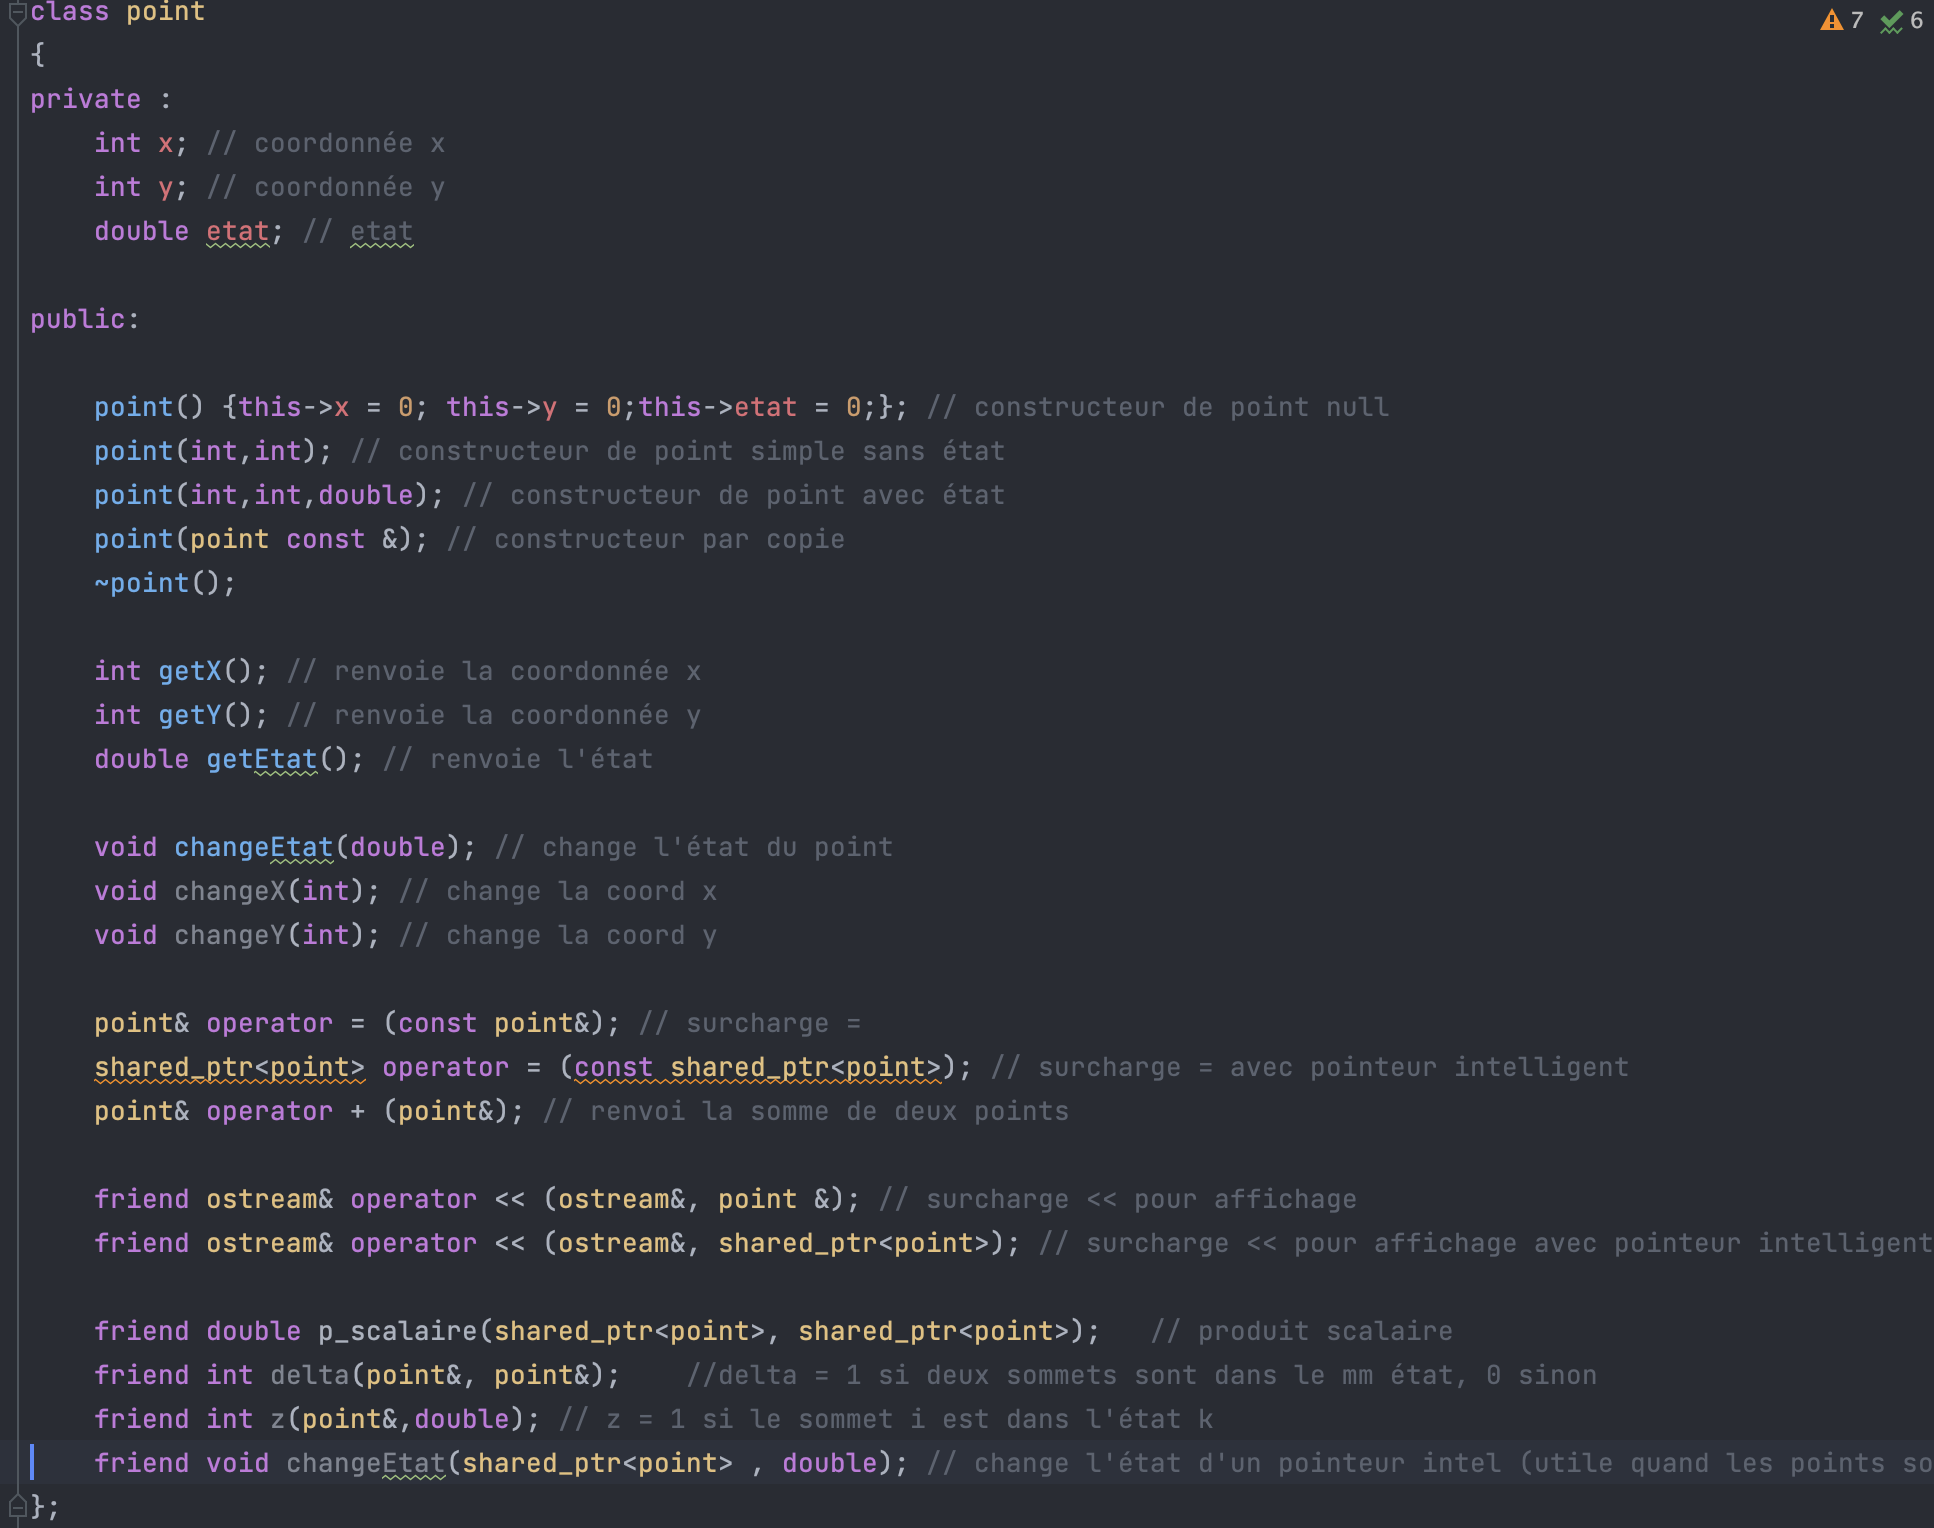
\includegraphics[width=0.9\textwidth, inner]{./img/prog/point/fichier_header_point}
        \caption{Header de la classe Point}
        \label{fig:prog2}
    \end{figure}
    ddzdz
\end{article}